\documentclass[12pt]{article}
\usepackage[margin=1in]{geometry}
\usepackage{amsmath}
\usepackage{graphicx}
\usepackage{xcolor}
\parindent=0pt
\begin{document}

\section*{Draw}

\verb$draw(f,x)$ draws a graph of function $f$ of $x$.

{\color{blue}
\begin{verbatim}
draw(x^2,x)
\end{verbatim}}

\begin{center}
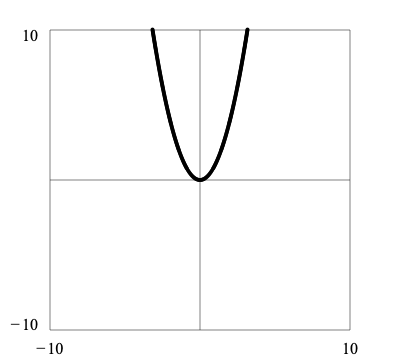
\includegraphics[scale=0.4]{parabola1.png}
\end{center}

The vectors \verb$xrange$ and \verb$yrange$ control the scale of the graph.

{\color{blue}
\begin{verbatim}
xrange = (-1,1)
yrange = (0,2)
draw(x^2)
\end{verbatim}}

\begin{center}
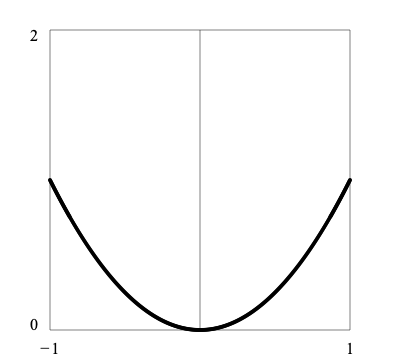
\includegraphics[scale=0.4]{parabola2.png}
\end{center}

Parametric drawing occurs when a function returns a vector.
The vector \verb$trange$ controls the parametric range.
The default is \verb$trange=(-pi,pi)$.
In the following example, \verb$draw$ varies \verb$theta$
over the default range $-\pi$ to $+\pi$.

{\color{blue}
\begin{verbatim}
xrange = (-10,10)
yrange = (-10,10)
f = 5 (cos(theta),sin(theta))
draw(f,theta)
\end{verbatim}}

\begin{center}
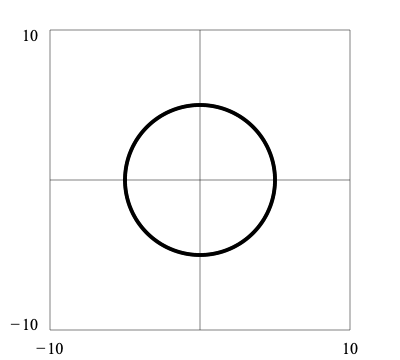
\includegraphics[scale=0.4]{circle1.png}
\end{center}

In the following example, \verb$trange$ is reduced
to draw a quarter circle instead of a full circle.

{\color{blue}
\begin{verbatim}
trange = (0,pi/2)
f = 5 (cos(theta),sin(theta))
draw(f,theta)
\end{verbatim}}

\begin{center}
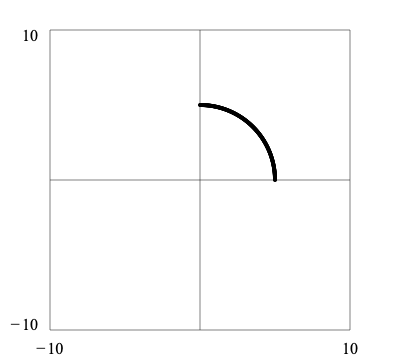
\includegraphics[scale=0.4]{circle2.png}
\end{center}

Draw a lemniscate.

{\color{blue}
\begin{verbatim}
trange = (-pi,pi)
X = cos(t) / (1 + sin(t)^2)
Y = sin(t) cos(t) / (1 + sin(t)^2)
f = 5 (X,Y)
draw(f,t)
\end{verbatim}}

\begin{center}
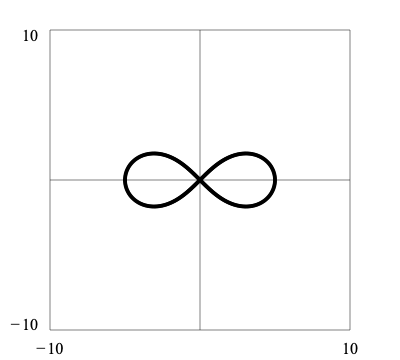
\includegraphics[scale=0.4]{lemniscate.png}
\end{center}

Draw a cardioid.

{\color{blue}
\begin{verbatim}
r = (1 + cos(t)) / 2
u = (cos(t),sin(t))
f = r u
xrange = (-1,1)
yrange = (-1,1)
trange = (0,2pi)
draw(f,t)
\end{verbatim}}

\begin{center}
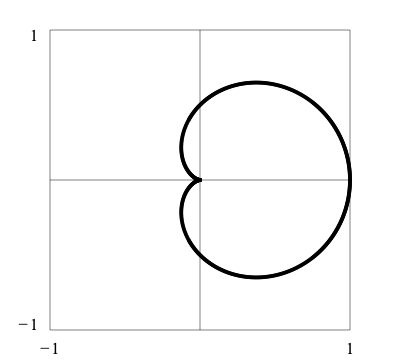
\includegraphics[scale=0.4]{cardioid.png}
\end{center}

\end{document}


\section*{Tricks}

\begin{enumerate}

\item
Use \verb$==$ to test for equality.
In effect, \verb$A==B$ is equivalent to \verb$simplify(A-B)==0$.

\item
In a script, line breaking is allowed where the scanner needs something to complete an expression.
For example, the scanner will automatically go to the next line after an operator.

\item
Setting \verb$trace=1$ in a script causes each line to be printed just before it is evaluated.
Useful for debugging.

\item
The last result is stored in symbol \verb$last$.

\item
Use \verb$contract(A)$ to get the mathematical trace of matrix $A$.

\item
Use \verb$binding(s)$ to get the unevaluated binding of symbol $s$.

\item
Use \verb$s=quote(s)$ to clear symbol $s$.

\item
Use \verb$float(pi)$ to get the floating point value of $\pi$.
Set \verb$pi=float(pi)$ to evaluate expressions with a numerical value for $\pi$.
Set \verb$pi=quote(pi)$ to make $\pi$ symbolic again.

\item
Assign strings to unit names so they are printed normally.
For example, setting \verb$meter="meter"$ causes the symbol \verb$meter$
to be printed as meter instead of $m_{eter}$.

\item
Use \verb$expsin$ and \verb$expcos$ instead of \verb$sin$ and \verb$cos$.
Trigonometric simplifications occur automatically when exponentials are used.

\end{enumerate}
\end{document}
